%=================
\chapter{Planning}
%=================

\section{Project Plan}
%---------------------

\subsection{Measurement of Project Effects}
Automatic generation of Lua scripts from c-header files would bring considerable resource savings in the customers usual work process. Time (and therefore financial resources) will be  be saved by delivery of the solution every time they need to know the contents of investigated IPC messages that include C struct(s).

The most of the savings will be caused by enabling filtering of the messages by the specific attribute in the C struct in Wireshark. Once this will be possible, a lot of unnecessary searching can be omitted.

Before the project start, C structs were investigated in two ways. The first, manual method, which means counting individual bytes of the binary file that includes data in C structs. This is possible only for small-sized messages. For bigger messages, this method is inapplicable, since the message can consist of several thousands bytes. The second method consists of writing the dissector (as Lua script) manually for the specific C header. Also, this method cannot be used for more complex C structs, i.e. those using nested structs. So far, there has been written about 10 Lua scripts manually.

According to the customer, there are approximately 3000 messages that include C structs and those need to be dissected by the solution. Time spent to write a dissector for a message manually depends on the struct’s complexity. For trivial messages, it takes 15 minutes to create a dissector manually. It took about 1 hour for the most complicated dissectors that were developed by the customer so far.

If 1 hour is the average time for creating a dissector for 1 message, our solution will save about 3000 hours of work. Due to everyday workload of the customer’s development team, this amount of time could never be used to accomplish such a task.

None of the workaround methods mentioned above is capable of processing messages with C structs that are big and complex. Time savings in these cases are not easily estimated.

Also, sometimes a representative of Thales Norway AS has to physically move to the their customer’s site to solve a problem. With the delivered solution, in some cases, this will be no longer necessary and the problem will be solved remotely by sending capture files to Thales and solving it in-house. Savings in this case are not only time-based but it will also directly cut the transportation costs and it will increase the satisfaction for the client.

\subsection{Limitations}
As in all other projects, the project members have to deal with various limitations and constraints given either by the customer or simply by the fact that they are students.

\subsubsection{Technical Limitations}
\begin{itemize}
	\item \textbf{C preprocessor:} To fulfill all the requirements we might need to either modify an existing preprocessor or write our own, which can be a huge undertaking.
	\item \textbf{Platforms:} SPARC platform that are required for the program are not available to the project group. 
\end{itemize}

\subsubsection{Non-technical Limitations}
\begin{itemize}
	\item \textbf{Experience:} None in the group has experience with Lua-scripts, running a project with larger team, or has planned a project before.
	\item \textbf{Time:} The project group has limited time of 12 weeks and a project deadline that cannot be changed. Also, the team consists of 7 members that have different schedules and so finding a time when everyone is available for a meeting might be difficult. These limitations might lead to considerable delays in the project progress.
	\item \textbf{Language:}         Language: In this project the team will have to write and speak in English, which is a second language for all team members. This may lead to misunderstandings and will negatively affect the time it takes to write the report.
\end{itemize}

\subsection{Tool Selection}
To support collaboration and project management the team has considered and selected the listed tools for use in this project.

\begin{itemize}
\item \textbf{Git \& Github:} 

The team has selected Git as the version control system, hosted at Github.com.

We had experience with CVS, SVN, Git and Mercurial, and although everyone knew SVN and only two knew Git, we selected Git for this project. We evaluated free hosting sites of version control systems, which could also provide us with other collaborative features that we wanted. github.com, bitbucket.com and sourceforge.net all provided wiki and issue tracker in addition to free version control system hosting. We eliminated sourceforge.net because their focus is divided between software users and developers, while the other two sites are fully focused on developers. The two remaining sites provides almost identical features, where one focuses on Git and the other on Mercurial.

Github with Git version control system was selected because more team members knew Git than Mercurial. By selecting a newer version control system like Git, we get advantageous features like branches and distributed repository model. Since we use different platforms, we will also use different git clients, but for Windows most of the group has selected tortoisegit.

\item \textbf{Skype:} 

Skype is an application which allows the user to make video and voice chats over the Internet, including conference calls and chatting. The team will use Skype to communicate and collaborate when we are not physically at the same location at the same time.

\item \textbf{Google Docs:} 

Google Docs is web-based office suite, which include documents, spreadsheets and presentations. It makes it possible to collaborate in real-time. For this project we are going to use Google Docs to collaborate on document drafts, and to share documents within the team and with the teams adviser.

\item \textbf{LaTeX}

LaTeX is a document markup language and document preparation system used to create reports, articles and books. LaTeX was chosen by the group for its high quality typesetting which produces professional looking documents, and because it is suitable for larger scientific reports. LaTeX also provides automatic numbering of chapter and sections, automatic generation of table of contents, cross-referencing and bibliography management. Since LaTeX files are plain text files they are suitable for versioning with a version control system like Git. We will use LaTeX to write the final project report, and we have created a few templates for test plans and minutes.

\item \textbf{Mailing list}

For asynchronous communication the team uses an electronic mailing list provided by IDI, NTNU.

\item \textbf{Google Calendar}

Since all team members have google accounts, we have created a google calendar to help schedule and keep track of meetings. A single calendar which all members can include in their own prevents misunderstandings and duplication of work.

\end{itemize}

\subsection{Based on the planned effort}
Calculations done by the course staff suggests that each student should use 325 person-hours distributed over 13 weeks. Our group, consisting of seven students, will have a total of 2275 person-hours to spend on the project. 

\subsection{Schedule of Results}
This project will have two deliveries, pre-delivery and final delivery.  The milestones and sprints are listed below. \newline
\textbf{Milestones} \newline
\begin{tabular}{l  l}
	30. August & Project start \\
	6. October & Pre-delivery of project report \\
	24. November & Final delivery of project report \\
	24. November & Presentation and project demo \\
\end{tabular}
\newline
\textbf{Sprints} \newline
\begin{tabular}{l  l}
	Sprint I & 14. September - 27. September \\
	Sprint II & 5. October - 18. October \\
	Sprint III & 19. October - 1. November  \\
	Sprint IV & 2. November - 15. November \\
\end{tabular}

\subsection{Concrete Project Work Plan}
The two first weeks on the project will be used on planning and pre study.
The project will be divided into 3 sprints, that will last for three weeks. Each sprint will have a total of 525 person-hours.
The last 1.5 week will be used to finish the final report and prepare for the presentation. 
Table \ref{tab:wbs} shows the work breakdown structure, and the project timeline is in figure \ref{fig:gantt}

\begin{table}[!ht] \footnotesize \center
\caption{Work Breakdown Structure\label{tab:wbs}}
\noindent\makebox[\textwidth]{%
\begin{tabularx}{\textwidth}{l l l c c}
	\toprule
	Task & From date & To date & Est Effort & Act Effort  \\
	\midrule
	Misc & 30.08.2011 & 24.11.2011 & 875 & 442 \\
	\midrule
	Project Management & 30.08.2011 & 24.11.2011 & 275 &132 \\
	Lectures & 02.09.2011 & 18.10.2011 & 100 & 60 \\
	Self Study & 30.08.2011 & 04.10.2011 & 150 & 42 \\
	Planning & 05.09.2011 & 12.09.2011 & 150 & 124 \\
	Pre-study & 05.09.2011 & 12.09.2011 & 100 & 32 \\
	Requirement Specification & 05.09.2011 & 12.09.2011 & 100 & 52 \\
	\midrule
	Sprint I & 14.09.2011 & 27.09.2011 & 200 & 112 \\
	\midrule
	Sprint I Planning & 14.09.2011 & 14.09.2011 & 30 & 27 \\
	Sprint I Work & 15.09.2011 & 26.09.2011 & 150 & 86 \\
	Sprint I Review & 27.09.2011 & 27.09.2011 & 20 & 0 \\
	\midrule
	Sprint II & 05.10.2011 & 18.10.2011 & 250 & 0 \\
	\midrule
	Sprint II Planning & 05.10.2011 & 05.10.2011 & 30 & 0 \\
	Sprint II Work & 06.10.2011 & 17.10.2011 & 200 & 0 \\
	Sprint II Review & 18.10.2011 & 18.10.2011 & 20 & 0 \\
	\midrule
	Sprint III & 19.10.2011 & 01.11.2011 & 250 & 0 \\
	\midrule
	Sprint III Planning & 19.10.2011 & 19.10.2011 & 30 & 0 \\
	Sprint III Work & 20.10.2011 & 31.10.2011 & 200 & 0 \\
	Sprint III Review & 01.11.2011 & 01.11.2011 & 20 & 0 \\
	\midrule
	Sprint IV & 02.11.2011 & 15.11.2011 & 250 & 0 \\
	\midrule
	Sprint IV Planning & 02.11.2011 & 02.11.2011 & 30 & 0 \\
	Sprint IV Work & 03.11.2011 & 14.11.2011 & 200 & 0 \\
	Sprint IV Review & 15.11.2011 & 15.11.2011 & 20 & 0 \\
	\midrule
	Report \& Presentation & 30.08.2011 & 24.11.2011 & 450 & 0 \\
	\midrule
	Write Report & 20.08.2011 & 24.11.2011 & 375 & 0 \\
	Presentation & 22.11.2011 & 24.11.2011 & 75 & 0 \\
	\midrule
	Total & 30.08.2011 & 24.11.2011 & 2275 & 553 \\
	\midrule
	\bottomrule
\end{tabularx}}
\end{table}

\begin{figure}[!ht]
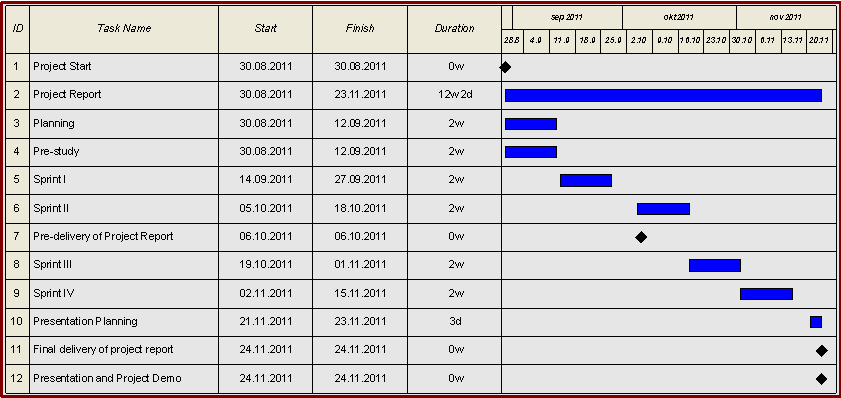
\includegraphics[scale=0.48]{./planning/img/gantt.png}
\caption{Gantt diagram}
\label{fig:gantt}
\end{figure}

\section{Project Organization}
%---------------------
This section describes how our group are organized.

\subsection{Project Organization}
Our project organization has a flat structure and the organization char can be seen in figure \ref{fig:orgchart}, the roles listed in the organization chart are described in table \ref{tab:roles}. \newline
\\
\begin{figure}[here]
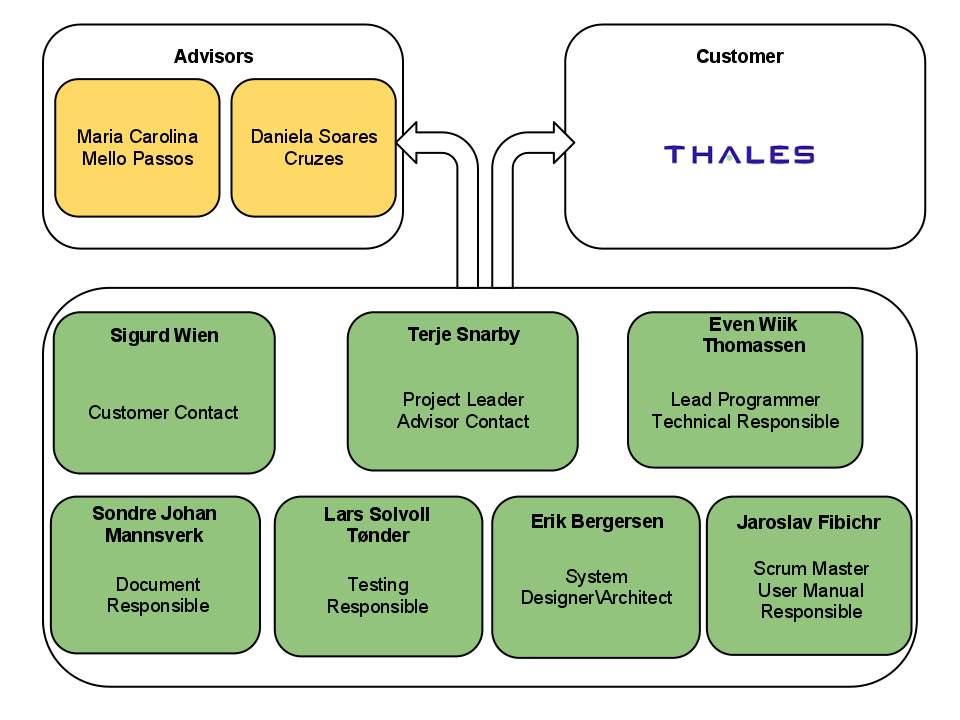
\includegraphics[scale=0.45]{./planning/img/organization.png}
\caption{Project Organization}
\label{fig:orgchart}
\end{figure}

\begin{table}[!ht] \footnotesize \center
\caption{Project Roles\label{tab:roles}}
\noindent\makebox[\textwidth]{%
\begin{tabularx}{\textwidth}{l X}
	\toprule
	Role name & Main responsibilities  \\
	\midrule
	Project manager & Responsible for having an overview of the project, delegating jobs and resolving conflicts. \\ 
	Adviser contact & Responsible for distributing information between the group and the adviser. \\
	Organizer & Responsible for setting up and informing the group about the meeting schedule. \\ 
	Document master & Responsible for document quality and quantity. \\ 
	System architect & The lead designer of the system. \\ 
	Lead programmer & Makes sure everyone follows the agreed code standards and ensures the quality of the code. \\ 
	Customer contact & Responsible for distributing information between the group and the customer. \\ 
	Technically responsible & Finds good technical solutions and makes sure that the essential tools are operative. \\ 
	Technology evangelist & Brings in ideas about new technologies and tools. \\ 
	Scrum master & Responsible for scrum meetings. \\ 
	Lead tester & Responsible for good test coverage, both unit and end to end, and to ensure the quality of those tests. \\ 
	Secretary & Takes note from each meetings and stores it in the cloud. Responsible for preparing minutes for adviser/customer. \\
	\bottomrule
\end{tabularx}}
\end{table}

\subsection{Partners}
This section lists the partners of this project. The customer of this project is Thales Norway AS, which are located at Lerkendal Stadium, Strindv 1, 7030 Trondheim.
The customer contacts are listed in table \ref{tab:part_cust}. The developers consists of seven student from NTNU, and are listed in table \ref{tab:part_dev}.  The project group has two advisers from  the Department of Computer and Information Science at NTNU, and are listed in table \ref{tab:part_adv}. \newline

\begin{table}[!ht] \footnotesize \center
\caption{Customers\label{tab:part_cust}}
\begin{tabular}{l l l}
	\toprule
	Name & Mobile & E-mail \\ 
	\midrule
	Christian Tellefsen & 959 98 765 & christian.telefsen@thalesgroup.com \\ 
	Stig Bjørlykke & 982 29 806 & stig.bjorlykke@thalesgroup.com \\ 
	\bottomrule
\end{tabular}
\end{table}

\begin{table}[!ht] \footnotesize \center
\caption{Developers\label{tab:part_dev}}
\begin{tabular}{l l l}
	\toprule
	Name & Mobile & E-mail  \\ 
	\midrule
	Terje Snarby & 915 27 390 & snarby@stud.ntnu.no \\ 
	Even Wiik Thomassen & 991 61 929 & evenwiik@stud.ntnu.no \\ 
	Sondre Johan Mannsverk & 948 15 506 & sondrejo@stud.ntnu.no \\ 
	Erik Bergersen & 917 48 305 & eribe@stud.ntnu.no \\ 
	Lars Solvoll Tønder & 976 00 317 & larssot@stud.ntnu.no \\ 
	Sigrud Wien & 472 54 625 & sigurdw@stud.ntnu.no \\ 
	Jaroslav Fibichr & 451 26 314 & jaroslaf@stud.ntnu.no \\ 
	\bottomrule
\end{tabular}
\end{table}

\begin{table}[!ht] \footnotesize \center
\caption{Advisers\label{tab:part_adv}}
\begin{tabular}{l l l}
	\toprule
	Name & Mobile & E-mail  \\ 
	\midrule
	Daniela Soares Cruzes & 942 49 891 & dcruzes@idi.ntnu.no \\ 
	Maria Carolina Mello Passos & & mariacm@idi.ntnu.no \\ 
	\bottomrule
\end{tabular}
\end{table}

\section{Quality Assurance}

\subsection{Routines for ensuring quality internally}
We will organize in pairs when producing items, where the pair reviews each others work. This is to try to find more errors and to get some extra perspective on style and solutions.

We also has assigned quality assurance responsibilities for three subjects: documents, code and tests. The respective team members will try to have a birds eye overview in their area to catch further errors.

We have agreed to have three weekly meetings to accommodate these routines.
\begin{itemize}
	\item Monday 12-14
	\item Wednesday 12-17
	\item Friday 10-13
\end{itemize}

\subsection{Phase result approval}
To ensure the quality of deliverable results, we have have, the group members responsible for quality assurance for a given subject will either read through, or delegate that that task to another free group member.

We will also present the results for the customer. They will then have an opportunity to point out problems and misunderstandings, and suggest solutions. We will then try to correct the problems and the reiterate the quality assurance.

\subsection{Procedures for customer meetings}
All customer meetings should be called with time, place, agenda specified. All background documents relevant to the meetings should also be supplied. This is to ensure efficient and effective meetings.

All customer meetings should be summarised in a document (minute). This document should include:
\begin{itemize}
	\item Time of meeting
	\item Place
	\item Meeting responsible
	\item Names of the attendees
	\item Decisions
	\item Actions
	\item Clarifications
	\item The above should be in sequence according to time
\end{itemize}

This summary should be done and sent to the customer by 12:00 the day after the meeting. If the customer does not approve the minutes, the minutes should again be corrected by and sent 12:00 the following day.

The customer contact is responsible for the above tasks.

The customer has committed to respond to our interactions within 2 working days.

\subsection{Procedure for advisor meeting}
A meeting with the adviser should be called before 14:00 the day before the meeting, and this calling should include:
\begin{itemize}
	\item Time
	\item Place
	\item Agenda
	\item Status report
	\item Table of reported working hours
	\item Minutes for the last meeting
	\item other relevant documents
\end{itemize}
The weekly adviser meeting will be at 10:30 every Friday unless otherwise stated.

The meetings should be summarized. The summary should include:
\begin{itemize}
	\item Time of meeting
	\item Place
	\item Version
	\item Names of the attendees
	\item Decisions
	\item Actions
	\item Clarifications
	\item A rough timeline of the above
\end{itemize}
The minutes should be written and sent before to the adviser for approval before 12:00 the day after the meeting. If the adviser should reject the minutes, they should be corrected and resent 12:00 the day following the rejection.

\subsection{Document templates and Standards}

\textbf{The group has created templates for:}
\begin{itemize}
	\item Meeting agenda
	\item Status report
	\item Meeting minutes
\end{itemize}
\textbf{Standard for organizing files:} \newline
We use GitHub and Google Docs to store the files included in this project. The location of a file is dependent on what type the file is. 
\begin{itemize}
	\item All source code is to be saved in the GitHub repository under source/. This ensures that all the team members have the current version of the code.
		\begin{verbatim}
CSjark/
    csjark/  -- todays source/, for source code
        test/  -- for unit tests
        etc/  -- for configuration files
        headers/  -- header files used to test the program
    bin/  -- file for executing our program
    docs/  -- for CSjark-specific documentation
    utils/  -- for cpp.exe and fake header files
		\end{verbatim}
	\item All textual documents that are completed will be put in the docs/ folder.
	\item All LaTeX documents are stored in the Github repository under report/.
\end{itemize}
\textbf{Standard for naming files:} \newline
The file name should consist of the name of the document(meeting minutes, agenda, phasedoc, e.g.) and the date, if applicable. \newline
\textbf{Standard for coding style:} \newline
The programming language used to implement the utility specified by the customer requirements are Python. The coding style the team has agreed upon is the Python Standard Styling Guide as defined by PEP8(LINK) (Python Enhancement Proposals \#8). In addition the design should attempt to be pythonic, as detailed by PEP20(LINK).

\subsection{Version Control Procedures}
Every relevant digital item should be pushed to our repository at github, and checked out by other participants. Those who works on a given item should commit and push their changes often, so that others can be as up to date as possible. All digital items should be labeled with a version number, starting at version 1. If an item goes under review and is deemed insufficient by the customer or  , the version number should also be incremented by one for each revision of the document

Relevant digital items includes source code, documents, picture files, binary blobs, etc.

NB: Google docs is not to be used for version control, so every document written there should also be pushed to git hub.

\subsection{Internal Reports}
Some of the groups internal activities should be documented. This includes:
\begin{itemize}
	\item Activities, what is done, and what remains
	\item Minutes for internal meetings
	\item Milestones, done/not done.
	\item Person-hours
\end{itemize}
These reports should follow the templates specified in Templates and Standards (A4) if applicable.

\section{Risk Management}

\textbf{R1. Choosing an incompatible technical solution} - The team decides to use a technical solution that is not suited for the given problem, or decides on an implementation that is too time consuming. \newline
\textbf{R2. Too much focus on report} -  We spend too much time working on the report and neglect the implementation. \newline
\textbf{R3. Too much focus on implementation} - We spend too much time working on the implementation and neglect writing all the needed documentation for the report. \newline
\textbf{R4. Illness/Absence} - Members of the team become ill or are otherwise unavailable. \newline
\textbf{R5. Conflicts within group} - Internal conflicts which are destructive to the groups ability to work together. \newline
\textbf{R6. Lack of technical competence} - The team lack the needed technical ability to solve the given problem. \newline
\textbf{R7. Miscommunication within team} - Team members don’t know what to do, or misunderstands the task given to them. \newline
\textbf{R8. Miscommunication with customer} - The team misunderstands the requirements given by the customer. \newline
\textbf{R9. Lack of experience with Scrum} - The team does not have any experience in doing Scrum projects. \newline

\begin{longtable}{l p{9cm}}
\caption{Handling Risks} \\
\endhead
\hline
\textbf{Nr} & R1 \\
\textbf{Risk factor} & Choosing an incompatible technical solution \\
\textbf{Consequences} & H: The project will not be completed on time, or at all. \\
\textbf{Probability} & M \\ 
\textbf{Strategy and actions} & Do a good pre-study, consult the customer’s technical expert. \\
\textbf{Deadline} & During the first sprint.\\
\textbf{Responsible} & Even and Erik \\
\hline
\textbf{Nr} & R2 \\
\textbf{Risk factor} & Too much focus on report \\
\textbf{Consequences} & M: The product will not be of a satisfying quality. \\
\textbf{Probability} & M \\ 
\textbf{Strategy and actions} & Plan enough hours to use on the customer product. Look at old reports for inspiration. Ask the adviser for help. \\
\textbf{Deadline} & Continuous\\
\textbf{Responsible} & Sondre \\
\hline
\textbf{Nr} & R3 \\
\textbf{Risk factor} & Too much focus on implementation \\
\textbf{Consequences} & H: The documentation will not be good enough, leads to a bad grade. \\
\textbf{Probability} & M \\ 
\textbf{Strategy and actions} & Plan enough hours to use on the report. Write documentation sooner later than later. Write good requirements that limit the scope of the project. \\
\textbf{Deadline} & Continuous \\
\textbf{Responsible} & All \\
\hline
\textbf{Nr} & R4 \\
\textbf{Risk factor} & Illness/Absence \\
\textbf{Consequences} & L/M/H: Consequences depend on how many members are absent, and how often they are absent. Absence may hinder the progress of the project in different ways.  \\
\textbf{Probability} & M \\ 
\textbf{Strategy and actions} & Make sure several people are proficient in the technical parts of the project. Have backups for the most important roles. \\
\textbf{Deadline} & Continuous \\
\textbf{Responsible} & Terje \\
\hline
\textbf{Nr} & R5 \\
\textbf{Risk factor} & Conflicts within group \\
\textbf{Consequences} & M: May lead to bad morale, which could affect the work of the team. Could also be a waste of time. \\
\textbf{Probability} & M \\ 
\textbf{Strategy and actions} & Not all conflicts are bad. If the conflict is simply a disagreement over technical issues, or the planning of the project, it could benefit the team. All such conflicts should lead to a constructive discussion that the entire team should take part in. Other types of conflicts, that can not positively influence the project should be avoided if possible. The team should agree on specific ground rules. \\
\textbf{Deadline} & Continuous \\
\textbf{Responsible} & Terje \\
\hline
\textbf{Nr} & R6 \\
\textbf{Risk factor} & Lack of technical competence \\
\textbf{Consequences} & H: The team is unable to solve the problem  \\
\textbf{Probability} & H \\ 
\textbf{Strategy and actions} & Make sure the team is proficient in the programming languages and tools that are to be used. Decide on technical solutions that the team already is familiar with. Do a good pre-study of the parts the team is unfamiliar with. Consult with the customer’s technical expert. \\
\textbf{Deadline} & Early phases of development (Pre-study, first sprint) \\
\textbf{Responsible} & All \\
\hline
\textbf{Nr} & R7 \\
\textbf{Risk factor} & Miscommuncation within team \\
\textbf{Consequences} & M: Team members waste time doing nothing, or doing something that is irrelevant. \\
\textbf{Probability} & M \\ 
\textbf{Strategy and actions} & Make sure that everyone knows what to do at all times. Ask questions if you are unsure about your specific task. \\
\textbf{Deadline} & Continuous \\
\textbf{Responsible} & Terje \\
\hline
\textbf{Nr} & R8 \\
\textbf{Risk factor} & Miscommunication with customer \\
\textbf{Consequences} & H: The team waste time on functionality the customer did not want. The completed product does not do what the customer wanted. \\
\textbf{Probability} & M \\ 
\textbf{Strategy and actions} & Make sure we and the customer have a common understanding of the requirements.
Have frequent meetings with the customers.  \\
\textbf{Deadline} & Continuous \\
\textbf{Responsible} & Sigurd \\
\hline
\textbf{Nr} & R9 \\
\textbf{Risk factor} & Lack of experience with Scrum \\
\textbf{Consequences} & M: The team does not provide the correct documents for the report, which could lead to a bad grade. \\
\textbf{Probability} & M \\ 
\textbf{Strategy and actions} & Learn how to properly do Scrum. Have Scrum meetings as often as possible. Get feedback on documents from adviser. \\
\textbf{Deadline} & Continuous \\
\textbf{Responsible} & Scrum Master \\
\hline
\label{tab:Risk}
\end{longtable}


